\documentclass[conference]{IEEEtran}
% Requires the standard IEEEtran class (part of any full TeX Live / MiKTeX
% install, or download from https://www.ctan.org/pkg/ieeetran). Swap to the
% target venue's official style file before final submission if it differs
% from a generic IEEE conference template.

\usepackage{cite}
\usepackage{amsmath}
\usepackage{amssymb}
\usepackage{amsfonts}
\usepackage{graphicx}
\usepackage{booktabs}
\usepackage{textcomp}
\usepackage{xcolor}
\usepackage{hyperref}
% placeins gives us \FloatBarrier, used below to stop figures from
% drifting past the section that introduces them -- without it, IEEEtran's
% two-column float algorithm can queue up every figure in a dense Results
% section and dump them all at the very end of the document.
% Loaded defensively: placeins ships with full TeX Live / MiKTeX and is
% present on the common online renderers, but NOT in a "basic" TeX Live
% install, where its absence is a fatal compile error rather than a merely
% degraded layout. The fallback makes \FloatBarrier a no-op so the document
% still compiles and still paginates correctly; only the float-drift
% guarantee is lost on that one uncommon setup. (Do NOT make the fallback
% \clearpage: it enforces the barrier but pads the paper from 7 pages to
% 11 by breaking a page at each of the four barriers.)
\IfFileExists{placeins.sty}
  {\usepackage{placeins}}
  {\providecommand{\FloatBarrier}{\par}}

% Marks a results-bearing value that does not exist yet. Never replace with
% an invented number; replace only with a real computed result.
\newcommand{\pending}[1]{\textcolor{red}{[PENDING: #1]}}

% The paper refers to several files in the project's source tree (the frozen
% spec, the model config, the decision log); this is where a reader finds them.
\newcommand{\repourl}{\url{https://github.com/reinamercy/Effective-Independence}}

% Marks a value that IS a real computed result, but from a run that has not
% yet reached full coverage (249/360 cells as of 2026-09-13; see
% Sec.~\ref{sec:results} and Limitations) -- flagged distinctly from
% \pending so a reader can tell "real but preliminary" apart from
% "not computed at all." Replace with \relax (i.e. remove the wrapper) once
% run_full_generation.py reports COMPLETE and these numbers are re-verified.
% Defined with \long\def rather than \newcommand so the argument may span a
% paragraph break -- several \prelim blocks now run to more than one
% paragraph, and a non-long macro fails there with the misleading
% "Paragraph ended before \@textcolor was complete".
% \textcolor is itself not \long, so passing multi-paragraph content to it
% fails even from a \long macro. A grouped \color declaration has the same
% visual effect and is transparent to paragraph breaks.
%
% TWO RENDERING MODES. Draft mode marks every preliminary value in blue with
% a dagger, which is useful while the numbers are still moving. Submission
% mode renders the same text plainly, because unexplained blue text and
% daggers read as an unfinished manuscript to a reviewer, and the
% partial-coverage caveat is already stated in prose at the head of
% Sec.~\ref{sec:results}, in every table and figure caption, and in
% Sec.~\ref{sec:limitations}. Switching modes changes no wording and no
% number. Set \prelimdrafttrue to go back to the marked-up version.
\newif\ifprelimdraft
\prelimdraftfalse
\makeatletter
\ifprelimdraft
  \long\def\prelim#1{{\color{blue}#1\,$^\dagger$}}
\else
  \long\def\prelim#1{#1}
\fi
\makeatother

\begin{document}

\title{Effective Independence: Quantifying the Reliability\\
Ceiling of Same-Base-Model LLM Ensembles}

\author{
\IEEEauthorblockN{Rahul Ramamoorthy}
\IEEEauthorblockA{\textit{UG Scholar} \\
\textit{Dept. of Computer Science \& Eng.} \\
\textit{Chennai Institute of Technology} \\
Chennai, India \\
\texttt{rahulramamoorthy.cse2023@citchennai.net}}
\and
\IEEEauthorblockN{Reina Mercy R}
\IEEEauthorblockA{\textit{UG Scholar} \\
\textit{Dept. of Computer Science \& Eng.} \\
\textit{Chennai Institute of Technology} \\
Chennai, India \\
\texttt{reinamercyr.cse2023@citchennai.net}}
}

\maketitle

\begin{abstract}
Debate, self-consistency, and LLM-as-judge pipelines assume ensemble
diversity they do not actually have when every voter is sampled from the
same base model. We apply the classical effective-sample-size statistic
$N_\text{eff}$ to this setting and measure it across four diversity axes commonly used to
build LLM ensembles (prompt, temperature, model size, and model family)
on three reasoning and factuality benchmarks: GPQA-Diamond, MATH levels 4-5,
and SimpleQA. \prelim{Measured with the usual correlation coefficient, even
$N=3$ ensembles behave like barely more than a single independent voter
($N_\text{eff}=1.09$ for prompt diversity, $1.51$ for model-family
diversity, $1.49$ for all 12 configurations together). We then show that
this coefficient flatters such ensembles, because it is bounded above by a
function of the two members' error rates: 11 of our 12 within-axis pairs sit
exactly at that bound. Looking at the error sets directly explains why. In
53 of 66 configuration pairs, one member's errors are a strict \emph{subset}
of the other's, so the weaker member recovers nothing the stronger one
missed and a majority vote has no material to work with. That nesting is
total for pairs drawn from a single base model (28 of 28) and falls to about
half for pairs spanning different labs (11 of 21), against a permutation
baseline of roughly 15\% ($p<0.0005$). The consequence is measurable at the
level practitioners care about: majority voting fails to beat the single
best member of its own ensemble on every axis we tested, and trails it by
12.5 points across all 12 configurations at twelve times the API cost.} We
recommend reporting the fraction of ensemble member pairs whose errors are
nested alongside any correlation-based diversity claim, since it is a direct
count that cannot be inflated by adding a weaker member.
\end{abstract}

\begin{IEEEkeywords}
large language models, ensemble diversity, self-consistency, LLM-as-judge,
multi-agent debate, effective sample size, reliability
\end{IEEEkeywords}

\section{Introduction}

\subsection{Background and Motivation}
Self-consistency decoding, multi-agent debate, and LLM-as-judge ensembles
all treat each sampled response as an independent vote. In practice, many
of these pipelines draw every sample from the same underlying base model,
varying only a shallow surface property such as the system prompt or the
sampling temperature. If those samples share correlated failure modes, the
effective diversity of the ensemble is far smaller than its nominal size
$N$ suggests. Majority voting, confidence aggregation, and judge panels
then inherit a reliability ceiling that is invisible to the people
building them.

\subsection{Challenges in Quantifying Ensemble Diversity}
Diversity is easy to induce along superficial axes (a different persona in
the system prompt, a higher decoding temperature) and hard to induce along
axes that plausibly decorrelate errors (a genuinely different training
run, a different base model family). Prior evaluation practice rarely
distinguishes between these axes' contribution to ensemble reliability, and
error correlation across ensemble members is rarely reported at all,
leaving practitioners without a way to tell whether adding a 4th or 8th
sample from the same model is buying real reliability or merely restating
the 1st sample with different words.

\subsection{Role of $N_\text{eff}$ in This Work}
We adapt the effective-sample-size framework used for correlated estimators
to LLM ensembles. The quantity is Kish's design effect~\cite{kish1965survey},
standard in survey sampling for discounting a nominal sample size by the
correlation among its units: given $N$ ensemble members with mean pairwise
error correlation $\bar\rho$,
\begin{equation}
N_\text{eff} = \frac{N}{1 + (N-1)\bar\rho}.
\label{eq:neff}
\end{equation}
$N_\text{eff}$ answers a concrete question: how many \emph{independent}
voters does this ensemble behave like? It also lets us compare diversity
axes on a common scale rather than only on raw accuracy. We compute
$N_\text{eff}$ for 12 configurations spanning 4 axes (3 configurations per
axis: prompt-diverse, temperature-diverse, size-diverse, and
family-diverse), with bootstrap confidence intervals over questions, and
report where each axis's $N_\text{eff}$ saturates as $N$ grows.

\subsection{Contributions}
\begin{itemize}
\item We decompose measured ensemble independence by \emph{construction
axis}, varying one practitioner-controllable choice at a time rather than
auditing diversity in aggregate.
\item We show the statistic normally used is biased in a specific,
correctable direction: $\phi$ is bounded above by a function of the members'
error rates (Eq.~\ref{eq:phimax}), so members differing in accuracy are
credited with independence they do not have. \prelim{11 of our 12 within-axis
pairs sit exactly at that bound.}
\item We identify the structure responsible: errors are largely
\emph{nested} rather than overlapping. \prelim{In 53 of 66 pairs one member's
errors are a strict subset of the other's, including all 28 same-base-model
pairs, against a permutation baseline of roughly 15\% ($p<0.0005$).} A nested
pair has zero complementary errors, so no aggregation rule over it can
recover a question.
\item We show the nesting rate falls monotonically as members become
genuinely more different \prelim{(100\%, 82\%, 52\% for pairs sharing a
model, sharing a lab, and spanning labs)}, which gives the practitioner
guidance a correlation ranking only gestures at.
\item We connect the structure to the outcome it predicts. \prelim{Majority
voting never beats the best member of its own ensemble on any axis, trailing
it by up to 25 points, and the number of questions a better aggregation rule
could have recovered is between 0 and 2 per ensemble.}
\item We compare five allocation strategies at equal API cost under all
three measures, and show that the ranking a correlation-based $N_\text{eff}$
would suggest does not survive the correction \prelim{(a 38\% apparent
advantage for cross-family ensembling becomes about 1\%)}. We release the
harness, the graded error matrix, and a decision log recording every
deviation from the frozen specification.
\end{itemize}

\section{Related Work}

Self-consistency decoding~\cite{wang2023selfconsistency} samples multiple
chain-of-thought~\cite{wei2022cot} completions from a single model and
takes a majority vote, implicitly treating the samples as independent
draws. Multi-agent debate frameworks~\cite{du2023debate} extend this to
multiple model instances arguing over several rounds, again typically
instantiated with a single underlying model. LLM-as-judge
evaluation~\cite{zheng2023judging} raises the same concern from the
evaluation side: a judge panel built from one base model may share the
judge's own biases across every panelist. A parallel line builds explicit LLM ensembles for accuracy: Agent
Forest~\cite{li2024moreagents} scales by sampling and voting over instances
of one model, and Mixture-of-Agents~\cite{wang2024moa} layers multiple LLMs.
Neither measures the pairwise error correlation its aggregation step relies
on, so a reported gain from more samples is not distinguishable, from the
published results alone, from the diminishing-returns pattern we measure in
Sec.~\ref{sec:results}.

Classical ensemble theory holds that accuracy gains are governed by the
trade-off between member accuracy and pairwise error correlation: the
ambiguity decomposition~\cite{krogh1994ambiguity} formalized it, and
Dietterich~\cite{dietterich2000ensemble} and Kuncheva and
Whitaker~\cite{kuncheva2003diversity} survey the constructions that induce
decorrelated errors and the diversity measures used to quantify them. We apply the same design-effect statistic to a setting that
theory did not anticipate: API-only, black-box ensembles whose members
cannot be inspected, retrained or explicitly decorrelated, only reconfigured
along the surface axes an API caller is given.

Two concurrent 2026 studies confirm the independence assumption is
unreliable, from different angles.
Kim~\cite{kim2026diversitymetrics} audits five diversity metrics across
31{,}900 ensemble subsets on MMLU-Pro and finds that apparent diversity
gains are largely capability entanglement rather than genuine error
decorrelation. Once capability is controlled for, simple majority voting
beats the best individual model in under 10\% of size-3 subsets.
Ding~\cite{ding2026agreement} audits cross-model agreement as a confidence
signal at large scale (265{,}000 samples on GPQA-Diamond and AIME) and
reports only weak correlation (0.20--0.59) between agreement and
correctness, concluding that self-consistency is a conditional proxy rather
than a standalone confidence score. Both results corroborate our starting
premise, that ensemble diversity is routinely overestimated, but neither
decomposes \emph{why}: they do not attribute the correlation they measure
to specific, practitioner-controllable construction choices.
Our contribution is narrower: we hold $N_\text{eff}$ fixed and vary one
structural axis at a time to localize \emph{where} an ensemble builder's
choices buy real independence. We also sharpen
Kim's~\cite{kim2026diversitymetrics} conclusion. That work attributes
apparent diversity gains to capability entanglement, established by
controlling for capability across ensemble subsets.
Sec.~\ref{sec:marginalbound} identifies a mechanism operating even within a
fixed subset: the correlation coefficient is itself bounded by the members'
error rates, so two members of unequal accuracy \emph{cannot} record high
correlation however similarly they fail. The entanglement is therefore a
property of the measurement, not only of the sampling, and it is
correctable.

\section{Methodology}

\subsection{Datasets}
We evaluate on three public benchmarks spanning multiple-choice and
free-response formats: GPQA-Diamond~\cite{rein2023gpqa}, a graduate-level
multiple-choice science benchmark; MATH~\cite{hendrycks2021math} restricted
to levels 4-5 (the hardest tier); and SimpleQA~\cite{wei2024simpleqa}, a
short-form factual QA benchmark. Free-tier API quotas (Sec.~\ref{sec:limitations})
constrained the question set to $N=30$ total (8 GPQA-Diamond, 11 MATH
levels 4-5, 11 SimpleQA), a deliberate reduction from an original target
of 800 questions. See \texttt{logs/decisions.md} for the two intermediate
reductions (800$\to$150$\to$30) and the quota measurements that drove each.

\subsection{Diversity Axes and Configurations}
We define 12 configurations across 4 diversity axes, 3 configurations per
axis, per the frozen specification in \texttt{config/project\_spec.yaml}:
\begin{itemize}
\item \textbf{Prompt-diverse}: one fixed model at temperature $0.7$, with
three system-prompt personas (``careful analyst'', ``confident expert'',
``skeptical reviewer'').
\item \textbf{Temperature-diverse}: the same fixed model and a neutral
prompt, at temperatures $\{0.3, 0.7, 1.0\}$.
\item \textbf{Size-diverse}: one model family, 3 sizes (small, medium,
flagship), neutral prompt, temperature $0.7$.
\item \textbf{Family-diverse}: 3 different model providers/labs, neutral
prompt, temperature $0.7$.
\end{itemize}
Each (question, configuration) pair receives exactly one sample, since the
goal is to measure cross-configuration error correlation rather than
within-configuration sampling variance. One consequence is worth stating
plainly: for the temperature axis, a single draw per configuration cannot
separate temperature-induced diversity from ordinary sampling noise at that
temperature, so that axis measures the diversity a practitioner actually
gets from one sample per setting rather than the full sampling distribution.

\subsection{Grading}
\label{sec:grading}
Each dataset is graded by its own deterministic procedure. GPQA-Diamond uses
exact match on the extracted answer letter. MATH uses symbolic equivalence
via \texttt{math\_verify} on the extracted \verb|\boxed{}| expression, so
that algebraically equal forms are not counted as disagreements. SimpleQA
uses normalized string containment against the reference answer, with an
LLM judge as a fallback only when containment fails.

That fallback deserves an explicit caveat, because the judge is
\texttt{gemini-3.5-flash}, which is also the base model behind 8 of the 12
configurations. A model therefore participates in grading responses that
include its own. We mitigate this three ways. The judge is a fallback rather
than the primary path, every invocation is written to an audit log released
with the paper, and, as a robustness check, we recompute the paper's main
result with SimpleQA excluded entirely (Sec.~\ref{sec:nesting}). We would
not use a self-judging setup by choice; it is a consequence of the free-tier
constraint that no second model with sufficient daily quota was available.

\subsection{Effective Independence Metric}
For any subset of configurations we compute the pairwise error-correlation
matrix and $N_\text{eff}$ via Eq.~\ref{eq:neff}, with 95\% confidence
intervals from 1{,}000 bootstrap resamples over questions. We additionally
report the fraction of questions on which $\geq$80\% of an ensemble agrees
and is wrong. This confident-correlated-error rate is the failure mode
majority voting cannot detect or correct. Finally, we compare a fixed set of five
allocation strategies at a matched budget of $k=3$ ensemble members
(Sec.~\ref{sec:budget}), which re-uses the cached results already
generated for the axis comparison and issues no additional API calls.

\subsection{Experimental Harness}
\label{sec:harness}
The harness, the frozen specification, the model configuration, the graded
error matrix, and the full decision log are released with this paper at
\repourl. File paths given below refer to that repository. The decision log
in particular records every deviation from the original specification, in
the order the deviations happened and with the reasoning at the time.

All generations are produced through a cached, rate-limited API client
(one persisted response per unique model/prompt/temperature/seed tuple),
so no (question, configuration) pair is ever re-queried. Every API call is
logged with the provider-returned model version string, token counts, and
cost. All generation uses the free-tier model set frozen in
\texttt{config/models.yaml}. The prompt- and temperature-diverse axes both
use \texttt{gemini-3.5-flash}~\cite{geminiteam2023}, which is also the
medium tier of size-diverse; the small and flagship tiers of size-diverse
are \texttt{gemini-3.5-\allowbreak flash-lite} and
\texttt{gemini-3.7-flash}~\cite{geminiteam2023}. Family-diverse combines
\texttt{gemini-3.5-flash}~\cite{geminiteam2023},
\texttt{z-ai/\allowbreak glm-5.2}~\cite{glmteam2026}, and
\texttt{nvidia/\allowbreak nemotron-3-\allowbreak ultra-550b-a55b}~\cite{nemotron2026ultra}.
(The OpenAI slot originally used
\texttt{openai/gpt-oss-20b} but was replaced with \texttt{z-ai/glm-5.2}
mid-project after OpenRouter permanently de-listed the former from its
free tier; see the decision log.) Dataset loading, configuration
construction, cached generation, per-dataset grading and $N_\text{eff}$
analysis are independently rerunnable modules connected only through on-disk
artifacts, so any stage can be re-run in isolation.

\FloatBarrier

\section{Results}
\label{sec:results}

\subsection{Quantitative Analysis}
\prelim{All results are computed on a fixed dataset of 249 graded
(question, configuration) cells, 69.2\% of the $30\times12$ design, at 73.1\%
overall accuracy. The absent cells were not dropped for any property of
their content: they are the cells a per-model daily API quota did not permit
us to collect (Sec.~\ref{sec:limitations}), so missingness is driven by
which model a configuration uses, not by question difficulty or by the
answers. Because coverage is still uneven, we report both what the uneven
data supports and what survives where every configuration is graded.} Table~\ref{tab:neff}
reports $N_\text{eff}$ per axis with bootstrap 95\% confidence intervals.
\prelim{Prompt-diverse and temperature-diverse, the two axes that vary
only a surface property of one fixed base model, show the highest mean
pairwise error correlation ($\bar\rho=0.87$ and $0.77$) and collapse to
$N_\text{eff}\approx 1.1$--$1.2$ regardless of their nominal size $N=3$.
Size-diverse (one family, three parameter scales) is only marginally
better ($\bar\rho=0.73$, $N_\text{eff}=1.22$), consistent with
\texttt{config/models.yaml}'s documented caveat that its ``flagship'' tier
is a newer Flash-generation model rather than a genuinely larger one, so
this axis likely understates what true parameter-scale diversity would
buy. Family-diverse scores best on this metric: mean error correlation
drops to $\bar\rho=0.50$ and $N_\text{eff}$ rises to $1.51$, still far
from the nominal $N=3$. We
deliberately stop short of calling this a
settled axis ranking. Under partial coverage the family-diverse advantage
rests on its two thinnest configuration pairs (Sec.~\ref{sec:pairdepth}),
and those same two pairs turn out to be constrained by a marginal bound
that accounts for their low correlation on its own
(Sec.~\ref{sec:marginalbound}). Extending this to the full 12-configuration ensemble, $N_\text{eff}$ rises
only from about 1.0 at $N=2$ to 1.49 at $N=12$: adding nine further
configurations buys roughly half of one additional effective voter.}

\begin{table}[!htb]
\centering
\caption{$N_\text{eff}$ per axis under $\phi$ (bootstrap 95\% CI) and under the marginal-robust $\bar{Q}$ (\prelim{249/360 cells}). $n_\text{min}$ is the fewest questions graded for both members of any pair in that axis. The $\phi$ columns are inflated by unequal member accuracy (Sec.~\ref{sec:marginalbound}).}
\label{tab:neff}
\begin{tabular}{lccccc}
\toprule
Axis & $\bar\rho$ & $N_\text{eff}(\phi)$ & 95\% CI & $\bar{Q}$ & $N_\text{eff}(Q)$ \\
\midrule
Prompt-diverse & 0.87 & 1.09 & [1.00, 1.29] & 1.00 & 1.00 \\
Temperature-div. & 0.77 & 1.18 & [1.00, 3.00] & 1.00 & 1.00 \\
Size-diverse & 0.73 & 1.22 & [1.03, 1.64] & 1.00 & 1.00 \\
Family-diverse & 0.50 & 1.51 & [1.06, 1.74] & 0.99 & 1.01 \\
\midrule
All 12 configs & 0.64 & 1.49 & [1.17, 1.90] & 0.95 & 1.04 \\
\bottomrule
\end{tabular}
\end{table}

\prelim{We also measure the confident-correlated-error rate: the fraction of
questions where $\geq$80\% of a $\geq$3-member ensemble is simultaneously
wrong. Across all 12 configurations this occurs on 5 of 30 eligible
questions (16.7\%), and per axis is highest for prompt-diverse (5/26,
19.2\%). A majority vote over any of these ensembles returns the wrong answer
confidently on those questions; diversity in surface presentation does not
protect against it. Per-configuration accuracy varies almost as much within
an axis as across axes (size-diverse spans 70\% to 89\%), which matters
because an axis can spread its members widely on accuracy and still have
highly correlated errors: $N_\text{eff}$ responds to \emph{which} questions
each member gets wrong, not how many.}

\FloatBarrier

\subsection{How Much Data Each Correlation Rests On}
\label{sec:pairdepth}
Each pairwise correlation is computed only over questions where \emph{both}
members are graded, and that overlap varies sharply.
\prelim{Seven of the twelve within-axis pairs rest on 8--9 shared questions,
two of them saturating at exactly $\rho=1.00$, which over nine questions is
more plausibly a small-sample artifact than a literal claim that two
configurations never disagree. The five well-sampled pairs ($n\geq26$) sit in
a much narrower band, $\rho=0.68$--$0.91$. This matters for the axis ranking:
family-diverse's advantage is driven by its two \emph{thinnest} pairs
($n=8$, $\rho=0.38$; $n=9$, $\rho=0.40$), while its only well-sampled pair
($n=27$) has $\rho=0.71$, squarely among the well-sampled same-base-model
pairs. Sec.~\ref{sec:nesting} therefore turns to a structural measure that
does not depend on estimating a coefficient at all.}

\subsection{Correlation Is Capped by Accuracy Differences}
\label{sec:marginalbound}
A second constraint limits what the correlation numbers can support, and it
cuts deeper than sample size. The phi coefficient between two binary error
vectors is bounded by their marginals. If configuration $A$ is wrong on a
fraction $p$ of questions and $B$ on a fraction $q$, with $p\leq q$, then
even when $A$'s errors are a strict subset of $B$'s, which is the most
concordant arrangement available,
\begin{equation}
\phi_{\max} = \sqrt{\frac{p\,(1-q)}{q\,(1-p)}},
\label{eq:phimax}
\end{equation}
which equals 1 only when $p=q$. The bound follows from maximising
$\phi = (n_{11}n_{00} - n_{10}n_{01})/\sqrt{pq(1-p)(1-q)}$ over the $2\times2$
tables compatible with fixed marginals: the numerator is largest when the
smaller error set is contained in the larger, which drives one off-diagonal
cell to zero and leaves Eq.~\ref{eq:phimax}. Two configurations with
different accuracy therefore \emph{cannot} record a high correlation,
however similarly they fail. A low $\phi$ is evidence of genuine error decorrelation only when it
sits appreciably below this ceiling.

\prelim{Checking each observed correlation against its own ceiling changes
how Table~\ref{tab:neff}
should be read. Eleven of the twelve within-axis pairs sit exactly at their
marginal-bound ceiling: their errors are already as correlated as their
differing accuracy permits. This includes both pairs responsible for
family-diverse's advantage, where one member is far more accurate than the
other ($p=0.12$ against $q=0.50$, and $p=0.11$ against $q=0.44$). At those
error rates Eq.~\ref{eq:phimax} caps $\phi$ at $0.378$ and $0.395$, and
those are precisely the observed values. The low correlation on this axis is
thus explained by its members having unequal accuracy, not by their failing
on complementary questions.

Exactly one of the twelve within-axis pairs falls clearly below its ceiling:
the two open-weight models, at $\phi=0.71$ against a bound of $0.86$. That
pair is also the best-sampled on its axis ($n=27$), and among the within-axis
pairs it is the only evidence of error decorrelation not attributable to an
accuracy mismatch. (Sec.~\ref{sec:nesting} widens the view to all 66 pairs,
where cross-lab pairs supply further such cases.) We therefore do not claim that cross-family ensembling
decorrelates errors. The defensible reading is narrower: measured
correlation is uniformly close to the maximum the data permits, and what
separates the axes in Table~\ref{tab:neff} is mostly how unequal their
members' accuracies are.

This does not undermine the $N_\text{eff}$ values themselves, which describe
the actual correlation structure whatever produces it, but it does undermine
any causal reading of the axis ranking. It is also a caution: an ensemble
can post a lower $\bar\rho$, and so a higher $N_\text{eff}$, simply by
including a weaker member.}

\subsection{Errors Are Nested, Not Complementary}
\label{sec:nesting}
The bound in Eq.~\ref{eq:phimax} is tight precisely when one member's errors
are a subset of the other's, so the finding that most pairs sit at their
ceiling is really a claim about the \emph{structure} of the error sets. That
structure can be counted directly, without estimating a coefficient at all,
and doing so turns out to be both more robust at this sample size and more
informative about what an ensemble can do.

Call a pair \emph{nested} when one member's error set contains the other's,
i.e. one of the two off-diagonal cells of the $2\times2$ error table is
empty. Pairs in which either member has no errors at all over the shared
questions are excluded rather than counted as nested, since such a member is
trivially contained in anything and would inflate the rate. Nesting is the case that matters operationally: if $A$'s mistakes are
a subset of $B$'s, then $B$ never answers a question correctly that $A$ gets
wrong, so no aggregation rule over $\{A,B\}$ can recover anything $A$ missed;
Sec.~\ref{sec:voting} tests that consequence directly against majority voting.
The pair is ordered by capability rather than diversified by it. A pair with
complementary errors on both sides, by contrast, gives a vote something to
work with.

\prelim{The result is stark. In 53 of 66 configuration pairs the errors are
fully nested (bootstrap 95\% CI over questions $[62\%, 98\%]$).
Table~\ref{tab:nesting} breaks this down by how genuinely
different the two members are, and the rate falls monotonically:
\textbf{all 28 pairs drawn from the same base model are nested}
(Wilson 95\% CI $[88\%, 100\%]$), against
82\% for pairs sharing a lab but not a model ($[59\%, 94\%]$), and 52\% for
pairs spanning different labs ($[32\%, 72\%]$). A Cochran--Armitage test
across the three ordered groups confirms the trend rather than leaving it to
the eye ($z=-4.12$, $p<10^{-4}$). Fig.~\ref{fig:nesting} plots the rates.

One scoping caveat belongs here, not only in Limitations. Eight of our
twelve configurations run on \texttt{gemini-3.5-flash}, so the same-model
row characterises one model observed under eight configurations rather than
a property established across many base models. Whether it generalises is an
open question our model set cannot answer.

Sparse tables could produce empty off-diagonal cells by luck, so this rate
means nothing without a baseline. We therefore permute, holding each
configuration's error count and its set of graded questions fixed and
shuffling only \emph{which} of those questions it fails. That destroys any
real shared failure mode while preserving the marginals and the coverage
pattern exactly. Over 2{,}000 permutations the expected nesting rate is
$15\%$ (95\% range $[8\%, 26\%]$) across all pairs and $16\%$ (95\% range
$[4\%, 32\%]$) among same-model pairs. The observed $80\%$ and $100\%$ are
roughly five times chance, and no permutation in either null reached the
observed value ($p<0.0005$). The nesting is a property of the models, not of
the sample size.

A second control addresses the grading circularity of
Sec.~\ref{sec:grading}. Excluding SimpleQA entirely leaves 19 questions and
21 defined pairs, where nesting is $86\%$ (18 of 21) and same-model pairs
remain fully nested (3 of 3). The effect is not produced by the self-judged
dataset, though that subset is small enough that we offer it only as a check
on direction.

The first row is the paper's sharpest result. Across every pair sharing a
base model there is not one question the second configuration gets right
that the first gets wrong. Changing persona or temperature reorders and
rewords the output, and changes how often the model is wrong, but never
contributes an independent success. That is a stronger and more checkable
claim than $\bar\rho=0.87$, and it does not rest on estimating a correlation
from nine questions.

It also explains the earlier numbers. Nested pairs are exactly those pinned
to the Eq.~\ref{eq:phimax} ceiling, so the $N_\text{eff}$ spread in
Table~\ref{tab:neff} largely tracks how unequal the members' accuracies are
while the underlying dependence is close to total throughout. Recomputing
with Yule's $Q$, which is not marginal-bounded and reaches 1 whenever an
off-diagonal cell is empty, makes this explicit: every axis falls to
$N_\text{eff}\approx1.0$ (Table~\ref{tab:nesting}), the 12-configuration
ensemble to $1.04$.

We are explicit about that substitution's status. Eq.~\ref{eq:neff} is
derived for a pairwise \emph{correlation}, and $Q$ sits on a different
scale, so $N_\text{eff}(Q)$ is a diagnostic rather than a drop-in estimator:
it shows that the ordering and magnitudes implied by $\phi$ do not survive a
measure free of the marginal cap. $Q$ also saturates at exactly 1 whenever an
off-diagonal cell is empty, so with six or seven errors in some pairs a
single flipped answer would move it. The nesting counts, which involve no
formula, therefore carry the claim; $N_\text{eff}(Q)$ expresses it on a
familiar scale. Both point the same way, and further than $\phi$ does.}

\begin{table}[!htb]
\centering
\caption{Error nesting (\prelim{249/360 cells}). A pair is nested when one member's errors are a subset of the other's, so the pair has no complementary errors for a vote to exploit.}
\label{tab:nesting}
\begin{tabular}{lcc}
\toprule
Pair type & Nested pairs & Rate \\
\midrule
Same exact model & 28 / 28 & 100\% \\
Same lab, different model & 14 / 17 & 82\% \\
Different lab & 11 / 21 & 52\% \\
\midrule
All pairs & 53 / 66 & 80\% \\
\bottomrule
\end{tabular}

\end{table}

\begin{figure}[!htb]
\centering
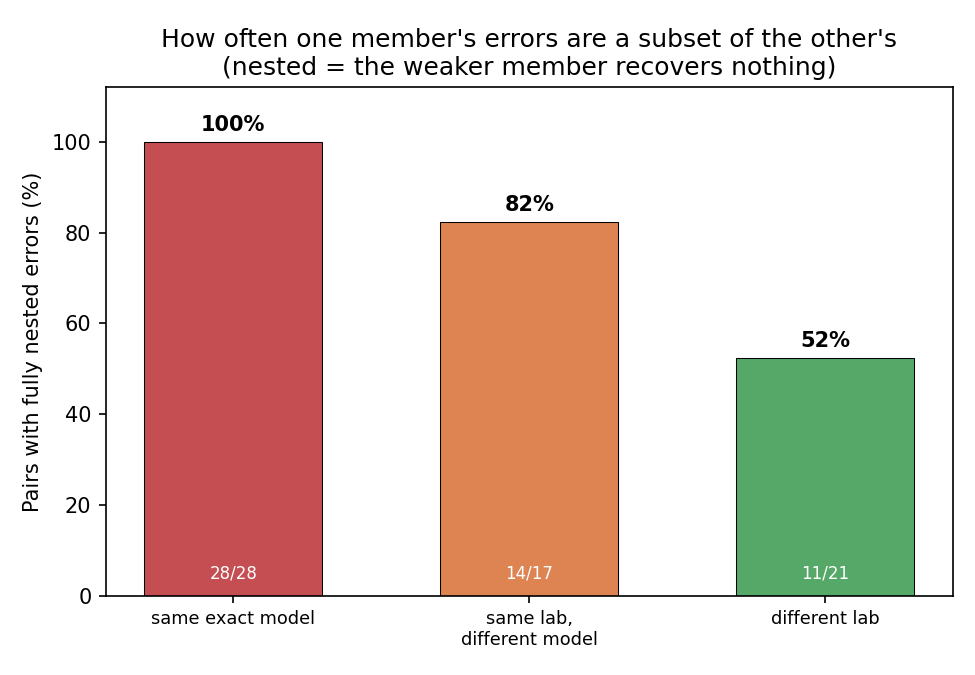
\includegraphics[width=\linewidth]{figures/nesting_by_pair_type.png}
\caption{How often one member's errors are a strict subset of the other's, by how genuinely different the two members are (\prelim{preliminary, 249/360 cells}).}
\label{fig:nesting}
\end{figure}

\FloatBarrier

\subsection{Does Majority Voting Actually Help?}
\label{sec:voting}
Everything above characterises the ensemble through a statistic or a
structure. Neither is what a practitioner buys. The question they face is
whether aggregating $k$ samples answers more questions correctly than using
one model, so we measure that directly. It requires no additional
generation: majority vote is computed from the same graded cells, with an
even split counted as incorrect. To keep the panel constant across
questions, each ensemble is scored only on questions where all of its
members are graded.

\prelim{Table~\ref{tab:voting} reports the result, and it is one-sided.
\textbf{Majority voting does not beat the single best member of its own
ensemble on any axis.} It loses by $3.8$ points on prompt-diverse, $11.1$ on
temperature-diverse and $25.0$ on family-diverse, and ties on size-diverse.
Over all 12 configurations together it reaches $75.0\%$ against $87.5\%$ for
the best member, a deficit of $12.5$ points at twelve times the API cost.

This is the outcome the nesting structure predicts. When one member's errors
are a subset of another's, the ensemble is ordered by capability, and a vote
can only dilute the strongest member with weaker ones that contribute no
question it missed. The recoverable column makes the size of the missed
opportunity explicit: across all five ensembles, the number of questions
where the majority was wrong while some member was right is 0 to 2. There is
very little for a better aggregation rule to find, so the failure is not a
deficiency of majority voting specifically. It is the absence of
complementary errors to aggregate.

The obvious objection is that the best member is identifiable only in
hindsight; a practitioner choosing in advance is more fairly compared against
the \emph{mean} member, which voting matches or beats everywhere except
family-diverse. The honest summary is narrower than ``voting is useless'':
voting recovers roughly the average member's accuracy, never an accuracy no
individual member already had.}

\begin{table}[!htb]
\centering
\caption{Majority vote against the members it aggregates (\prelim{249/360 cells}). ``Recov.'' counts questions where the majority was wrong but at least one member was right. A non-positive vote${-}$best column means voting never beat the strongest member.}
\label{tab:voting}
\begin{tabular}{lccccc}
\toprule
Ensemble & $n_q$ & Vote & Best & Mean & Recov. \\
\midrule
Prompt-diverse & 26 & 76.9 & 80.8 & 76.9 & 1 \\
Temperature-diverse & 9 & 77.8 & 88.9 & 81.5 & 1 \\
Size-diverse & 9 & 88.9 & 88.9 & 81.5 & 0 \\
Family-diverse & 8 & 62.5 & 87.5 & 62.5 & 2 \\
\midrule
All 12 configs & 8 & 75.0 & 87.5 & 71.9 & 1 \\
\bottomrule
\end{tabular}
\end{table}

\subsection{Budget-Matched Allocation}
\label{sec:budget}
The axis comparison above asks which kind of diversity decorrelates errors.
The question a practitioner actually faces is narrower: given a fixed
number of API calls per question, how should they be spent? We therefore
compare five allocation strategies at a matched budget of $k=3$ calls.
Every strategy issues exactly the same number of requests, so any
difference in $N_\text{eff}$ is attributable purely to how the budget was
allocated rather than to how large it was.

We note explicitly that the frozen specification framed this comparison as
one at matched total API \emph{cost}. Every model in the final
configuration is free-tier, so dollar cost cannot be the matching
variable; we match on $k$ instead, which is both the genuinely scarce
resource in this project (per-model daily request quotas) and the quantity
a practitioner controls. This substitution is recorded in
\texttt{logs/decisions.md} rather than made silently.

Table~\ref{tab:budget} reports each allocation under all three measures.
Reporting only the $\phi$ column here would contradict
Sec.~\ref{sec:marginalbound}, and the disagreement between the columns is
large enough that it changes the conclusion.

\prelim{Read through $\phi$, cross-family looks decisively best:
$N_\text{eff}=1.51$ against $1.09$ for three prompts of one model, a 38\% gain
at identical cost. Almost all of that gap is the accuracy artifact. Under
$Q$ the same comparison is $1.01$ against $1.00$. We therefore do not claim a
38\% reliability gain from crossing model families, and a practitioner should
not budget for one.

What survives the correction is categorical, and visible in the last column.
Every allocation built from a single base model is fully nested, 3 pairs of
3: no member ever answers a question its partners miss. The two allocations
spanning more than one model each contain exactly one pair with
complementary errors. That is the real distinction at a fixed budget, and it
is a difference in kind, not a 38\% improvement in a statistic.

This also corrects a reading $\phi$ invites. Under $\phi$ the mixed
allocation ($1.17$) looks far worse than cross-family ($1.51$), suggesting
that spreading a budget across axes poorly substitutes for changing model
family. Under $Q$ the two are indistinguishable ($1.01$ each) and both
contain one complementary pair. What matters is whether the allocation spans
more than one base model at all, not how many \emph{kinds} of diversity it
mixes. With three effective ties and $N=30$, we cannot rank the non-nested
allocations against each other and do not attempt to.}

\begin{table}[!htb]
\centering
\caption{Allocations at a matched budget of $k=3$ API calls per question (\prelim{preliminary, 249/360 cells}). Every row costs the same. The $\phi$ column overstates the spread because it is capped by differences in member accuracy (Sec.~\ref{sec:marginalbound}); the $Q$ and nesting columns are the ones to read.}
\label{tab:budget}
\begin{tabular}{lccc}
\toprule
Allocation ($k=3$) & $N_\text{eff}(\phi)$ & $N_\text{eff}(Q)$ & Nested \\
\midrule
Same model, 3 prompts & 1.09 & 1.00 & 3/3 \\
Same model, 3 temperatures & 1.18 & 1.00 & 3/3 \\
Same family, 3 sizes & 1.22 & 1.00 & 3/3 \\
\midrule
Mixed, one per axis & 1.17 & 1.01 & \textbf{2/3} \\
3 different families & 1.51 & 1.01 & \textbf{2/3} \\
\bottomrule
\end{tabular}
\end{table}

\FloatBarrier

\section{Limitations}
\label{sec:limitations}
\textbf{Model set.} Budget constraints limited us to free-tier providers
(Sec.~\ref{sec:harness}) rather than the closed-frontier set originally
planned, after we found the real free-tier quota (20 requests/day/model) far
below what public documentation reports. Family-diverse therefore mixes
closed-weight (Gemini) and open-weight (GLM, Nemotron) models rather than
three frontier flagships, and its members are the most unequal in accuracy
of any axis, which interacts with the bound below.
\textbf{Dataset size.} At $N=30$ questions ($\sim$8--11 per dataset) some
95\% intervals span nearly their whole range (temperature-diverse:
$[1.00,3.00]$). This is a power limitation, not an artifact of the method,
so results should be read as a pilot. Intervals tighten as coverage grows
(prompt-diverse moved from $[1.00,3.00]$ at 205/360 cells to $[1.00,1.29]$ at
249/360) but will not all become informative at $N=30$.
\textbf{Uneven coverage.} Missing cells concentrate in the eight
configurations sharing one model's quota, so graded counts range from 9 to 30
and most pairs rest on 8--9 shared questions. Cross-axis comparisons are
therefore confounded with coverage. \prelim{A complete-case analysis removes
the confound but leaves only 8 of 30 questions with all twelve
configurations graded, too few to rank four axes; we report the all-12
voting result on those 8 questions (Table~\ref{tab:voting}) and otherwise
decline to rank.} Table~\ref{tab:neff} is descriptive of this dataset, not a
population ordering.
\textbf{Both association measures are constrained.} $\phi$ cannot exceed the
Eq.~\ref{eq:phimax} ceiling and \prelim{11 of 12 within-axis pairs sit
exactly there}, so differences in $\bar\rho$ largely track how unequal member
accuracies are; a design holding accuracy constant would separate the
effects, but the free-tier set fixes which models exist at each tier. $Q$
conversely saturates at 1 whenever an off-diagonal cell is empty, and with
six or seven errors in some pairs one flipped answer would move it. The
nesting counts are immune to both problems.
\textbf{Nesting is pairwise.} Three configurations can be pairwise nested in
a chain with no single member dominating all others; our counts do not
distinguish that case, and the operational claim we make is the pairwise one.
\textbf{Single sample per cell.} We measure cross-configuration correlation,
not within-configuration sampling variance, so for the temperature axis in
particular one draw per setting cannot separate temperature-induced
diversity from sampling noise.
\textbf{A grading judge shares a base model with the configurations.}
SimpleQA falls back to an LLM judge when string containment fails, and that
judge is \texttt{gemini-3.5-flash}, which underlies 8 of the 12
configurations (Sec.~\ref{sec:grading}). Excluding SimpleQA leaves the
nesting result intact \prelim{(86\% overall, same-model pairs still fully
nested)}, so we do not believe it drives the finding, but an independent
grader would be preferable and was unavailable within the quota.

\section{Conclusion}
\prelim{On the data collected here, prompt- and temperature-diversity are the
cheapest and most commonly used axes, and the two that buy the least real
independence: $N_\text{eff}\approx 1.1$--$1.2$ at nominal $N=3$. Model-family
diversity is the axis on which measured correlation falls furthest, but we
do not claim the gain its $\phi$-based $N_\text{eff}$ of $1.51$ implies: that
margin rests on the thinnest pairs (Sec.~\ref{sec:pairdepth}) and on pairs
whose low correlation is already explained by unequal member accuracy
(Sec.~\ref{sec:marginalbound}). Corrected, the comparison is $1.01$ against
$1.00$.

The ranking is the least robust part of these results. The sturdiest finding
is structural and needs no coefficient: in 53 of 66 pairs one member's
errors are a strict subset of the other's, including every pair drawn from
the same base model. Where errors are nested there is nothing to recover,
which is why a nominal three or twelve votes behaves like roughly one. The
prediction is borne out directly: majority voting never beat the best member
of its own ensemble, and only 0 to 2 questions per ensemble were even
available for a smarter aggregator to rescue.

For debate, self-consistency, and judge-panel pipeline design, that means
scaling the number of same-base-model samples is a much weaker reliability
lever than its nominal $N$ suggests. At a fixed budget the distinction our
data supports is categorical rather than a matter of degree: allocations
drawn entirely from one base model are fully nested and can recover nothing,
while allocations spanning more than one base model contain at least one
pair with complementary errors. How many different \emph{kinds} of diversity
are mixed matters less than whether the base model changes at all.

Measuring that structure carries its own trap: because $\phi$ is capped by
the members' error rates, an ensemble can report a flattering $N_\text{eff}$
merely by including a weaker member. The remedy needs no extra API calls.
Alongside any reported $\bar\rho$ or $N_\text{eff}$, publish the fraction of
member pairs whose errors are nested: a direct count, uninflatable by adding
a weak member, answering what a builder needs to know.

These are pilot-scale results (Sec.~\ref{sec:limitations}), consistent in
direction with classical ensemble theory and with concurrent independent
work~\cite{kim2026diversitymetrics,ding2026agreement}. The magnitudes, and
the axis ranking especially, remain provisional until coverage is complete.
The nesting result is the one we expect to survive, since further coverage
can only add questions on which a member might differ, and 28 of 28
same-model pairs have produced none so far.}

% Bibliography is embedded directly (rather than via \bibliography +
% bibtex) so the document compiles correctly in a single pdflatex pass on
% any renderer, including ones that do not run a separate bibtex/biber
% step. The same 20 entries also live in references.bib in bibtex-ready
% form for anyone whose toolchain does run bibtex -- keep both in sync if
% a reference changes.
\begin{thebibliography}{18}

\bibitem{wang2023selfconsistency}
X. Wang, J. Wei, D. Schuurmans, Q. Le, E. Chi, S. Narang, A. Chowdhery, and D. Zhou, ``Self-Consistency Improves Chain of Thought Reasoning in Language Models,'' in \emph{International Conference on Learning Representations (ICLR)}, 2023.

\bibitem{wei2022cot}
J. Wei, X. Wang, D. Schuurmans, M. Bosma, B. Ichter, F. Xia, E. H. Chi, Q. V. Le, and D. Zhou, ``Chain-of-Thought Prompting Elicits Reasoning in Large Language Models,'' in \emph{Advances in Neural Information Processing Systems (NeurIPS)}, 2022, pp. 24824--24837.

\bibitem{du2023debate}
Y. Du, S. Li, A. Torralba, J. B. Tenenbaum, and I. Mordatch, ``Improving Factuality and Reasoning in Language Models through Multiagent Debate,'' \emph{arXiv preprint arXiv:2305.14325}, 2023.

\bibitem{zheng2023judging}
L. Zheng, W.-L. Chiang, Y. Sheng, S. Zhuang, Z. Wu, Y. Zhuang, Z. Lin, Z. Li, D. Li, E. P. Xing, H. Zhang, J. E. Gonzalez, and I. Stoica, ``Judging LLM-as-a-Judge with MT-Bench and Chatbot Arena,'' in \emph{Advances in Neural Information Processing Systems (NeurIPS)}, 2023.

\bibitem{li2024moreagents}
J. Li, Q. Zhang, Y. Yu, Q. Fu, and D. Ye, ``More Agents Is All You Need,'' \emph{Transactions on Machine Learning Research}, 2024.

\bibitem{wang2024moa}
J. Wang, J. Wang, B. Athiwaratkun, C. Zhang, and J. Zou, ``Mixture-of-Agents Enhances Large Language Model Capabilities,'' \emph{arXiv preprint arXiv:2406.04692}, 2024.

\bibitem{kish1965survey}
L. Kish, \emph{Survey Sampling}. New York, NY, USA: John Wiley \& Sons, 1965.

\bibitem{krogh1994ambiguity}
A. Krogh and J. Vedelsby, ``Neural Network Ensembles, Cross Validation, and Active Learning,'' in \emph{Advances in Neural Information Processing Systems (NIPS)}, 1994, pp. 231--238.

\bibitem{dietterich2000ensemble}
T. G. Dietterich, ``Ensemble Methods in Machine Learning,'' in \emph{International Workshop on Multiple Classifier Systems}, 2000, pp. 1--15.

\bibitem{kuncheva2003diversity}
L. I. Kuncheva and C. J. Whitaker, ``Measures of Diversity in Classifier Ensembles and Their Relationship with the Ensemble Accuracy,'' \emph{Machine Learning}, vol. 51, no. 2, pp. 181--207, 2003.

\bibitem{kim2026diversitymetrics}
D. Kim, ``Are Diversity Metrics Measuring Diversity? A Capability-Controlled Audit of Majority-Vote Gain in LLM Ensembles,'' \emph{arXiv preprint arXiv:2607.20768}, 2026.

\bibitem{ding2026agreement}
K. Ding, ``When LLMs Agree, Are They Right? Auditing Self-Consistency and Cross-Model Agreement as Confidence Signals,'' \emph{arXiv preprint arXiv:2607.08065}, 2026.

\bibitem{rein2023gpqa}
D. Rein, B. L. Hou, A. C. Stickland, J. Petty, R. Y. Pang, J. Dirani, J. Michael, and S. R. Bowman, ``GPQA: A Graduate-Level Google-Proof Q\&A Benchmark,'' \emph{arXiv preprint arXiv:2311.12022}, 2023.

\bibitem{hendrycks2021math}
D. Hendrycks, C. Burns, S. Kadavath, A. Arora, S. Basart, E. Tang, D. Song, and J. Steinhardt, ``Measuring Mathematical Problem Solving With the MATH Dataset,'' in \emph{Advances in Neural Information Processing Systems (NeurIPS) Datasets and Benchmarks Track}, 2021.

\bibitem{wei2024simpleqa}
J. Wei, N. Karina, H. W. Chung, Y. J. Jiao, S. Papay, A. Glaese, J. Schulman, and W. Fedus, ``Measuring Short-Form Factuality in Large Language Models,'' \emph{arXiv preprint arXiv:2411.04368}, 2024.

\bibitem{geminiteam2023}
Gemini Team, ``Gemini: A Family of Highly Capable Multimodal Models,'' \emph{arXiv preprint arXiv:2312.11805}, 2023.

\bibitem{glmteam2026}
GLM Team, A. Zeng \emph{et al.}, ``GLM-5: from Vibe Coding to Agentic Engineering,'' \emph{arXiv preprint arXiv:2602.15763}, 2026.

\bibitem{nemotron2026ultra}
NVIDIA, ``Nemotron 3 Ultra: Open, Efficient Mixture-of-Experts Hybrid Mamba-Transformer Model for Agentic Reasoning,'' \emph{arXiv preprint arXiv:2606.15007}, 2026.

\end{thebibliography}

\end{document}
